\documentclass[12pt, a4paper]{report}
\usepackage[utf8]{inputenc}
\usepackage{graphicx}
\usepackage{nameref}
\graphicspath{ {Pictures/} }
\usepackage{hyperref}
\hypersetup{
    colorlinks=true,
    linkcolor=blue,
    filecolor=magenta,      
    urlcolor=red,
}
\usepackage{geometry}
\usepackage{float}
\usepackage{algorithm}
\usepackage{algpseudocode}
\usepackage{amsmath, bm}
\usepackage[export]{adjustbox}
\usepackage{subcaption}
\usepackage{mathabx}
 

\title{%  
Homework Assignment 4: \\
Trajectory Planning
   \\
  \large  Dynamics Of Non Linear Robotic Systems}
\author{Ilia Sevostianov %\thanks{thanks to God}
    }
\date{\today}

\begin{document}
	\maketitle

\tableofcontents
\newpage

\section*{Code}
\addcontentsline{toc}{section}{\protect\numberline{}Code}%

The code with comments you can find \href{https://github.com/Terminateit/DynamicsHA4.git}{here}.

\section*{Task 1}
\addcontentsline{toc}{section}{\protect\numberline{}Task1}%

Compute the joint trajectory from $q(0) = 1$ to $q(2) = 4$ with null initial and final velocities:
\begin{enumerate}
	\item  Use polynomial position profile
	\item  Use trapezoidal velocity profile.
	\item  Use velocity profile of the type $\dot{q}(t) = a(b + sin(ct))$.
\end{enumerate}

The problem of trajectory planning is to find a trajectory that connects an
initial to a final configuration while satisfying other specified constraints at
the endpoints (e.g., velocity and/or acceleration constraints).

{\centering
\subsection*{Polynomial Position Profile} \label{sec: 1Poly}
}
\addcontentsline{toc}{subsection}{\protect\numberline{}Polynomial position profile}%

We have four constraints to satisfy:
\begin{itemize}
	\item $q(0) = 1$
	\item $q(2) = 4$
	\item $\dot{q}(0) = 0$
	\item $\dot{q}(2) = 0$
\end{itemize}

So, we require a polynomial with four
independent coefficients that can be chosen to satisfy these constraints. Thus
we consider a cubic trajectory of the form:
\begin{equation}
	q(t) = a_0 + a_1t + a_2t^2 + a_3t^3
	\label{eqn:traj}
\end{equation}

Then, velocity $\dot{q}(t)$ and accelerations $\ddot{q}(t)$ equations are:
\begin{equation}
	\dot{q}(t) = a_1 + 2a_2t + 3a_3t^2	
	\label{eqn:vel}
\end{equation}

\begin{equation}
	\ddot{q}(t) = 2a_2t + 6a_3t	
\end{equation}

Combining equations \ref{eqn:traj} and \ref{eqn:vel} with the four constraints yields four
equations in four unknowns:
\begin{equation}
	q(0) = a_0 + a_1t_0 + a_2t_0^2 + a_3t_0^3
\end{equation}
\begin{equation}
	\dot{q}(0) = a_1 + 2a_2t_0 + 3a_3t_0^2
\end{equation}

\begin{equation}
	q(2) = a_0 + a_1t_f + a_2t_f^2 + a_3t_f^3
\end{equation}
\begin{equation}
	\dot{q}(2) = a_1 + 2a_2t_f + 3a_3t_f^2
\end{equation}

These four equations can be combined into a single matrix equation

\begin{equation}
	\begin{bmatrix}
	1 \ t_0 \ t_0^2 \ t_0^3 \\
	0 \ 1 \ 2t_0 \ 3t_0^2 \\
	1 \ t_f \ t_f^2 \ t_f^3 \\
	0 \ 1 \ 2t_f \ 3t_f^2 \\
	\end{bmatrix}
	\begin{bmatrix}
	a_0 \\ a_1 \\ a_2 \\ a_3 \\
	\end{bmatrix} = 
	\begin{bmatrix}
	q(0) \\ \dot{q}(0) \\ q(2) \\ \dot{q}(2) \\
	\end{bmatrix}
	\label{eq:matrix}
\end{equation}

The equation \ref{eq:matrix} can be written as:

\begin{equation}
	Ma = b
\end{equation}

Thus, we can find the coefficients of polynomial trajectory.

\begin{equation}
	a = M^{-1}b
	\label{eg:inverse}
\end{equation}

That's the main idea how to solve such trajectory planning tasks. And the polynomial equation's power depends on amount of constraints. All the coefficients can be found through equation \ref{eg:inverse}.

So, polynomial position profile for given constraints is:

\begin{equation}
q(t) = -\frac{3t^3}{4} + \frac{9t^2}{4} + 1
\end{equation}
graphs of trajectory you can see in the figure \ref{fig:mesh1}
\begin{figure}[H]
	\centering
		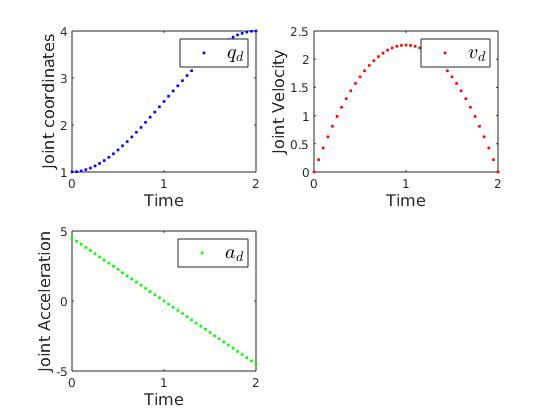
\includegraphics[width=0.6\textwidth]{11} % File
	\caption{the joint trajectory from $q(0) = 1$ to $q(2) = 4$ (polynomial)} % Name
	\label{fig:mesh1}
\end{figure}


{\centering
\subsection*{Trapezoidal Velocity Profile} \label{sec: 1Trap}
}
\addcontentsline{toc}{subsection}{\protect\numberline{}Trapezoidal Velocity Profile}%

This type of trajectory is appropriate when a constant velocity is desired along a portion of the path. The LSPB
trajectory is such that the velocity is initially “ramped up” to its desired value
and then “ramped down” when it approaches the goal position.

The first part from time $t_0$ to
time $t_b$ is a quadratic polynomial. This results in a linear “ramp” velocity. At
time $t_b$ , called the \textbf{blend time}, the trajectory switches to a linear function. This corresponds to a constant velocity. Finally, at time $t_f - t_b$ the trajectory switches once again, this time to a quadratic polynomial so that the velocity is linear.

Let's say, we have the graph for LSPB trajectory (velocity graph, figure \ref{fig:mesh2}).

\begin{figure}[H]
	\centering
		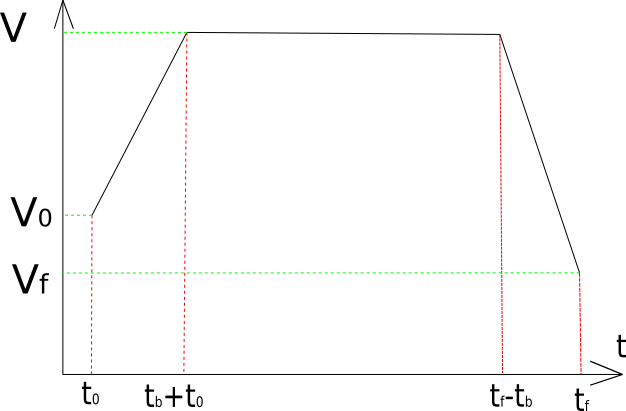
\includegraphics[width=0.8\textwidth]{trapezia} % File
	\caption{Trapezoidal velocity profile} % Name
	\label{fig:mesh2}
\end{figure}

So, we have:
\begin{equation}
q = \begin{cases} 
      a_{10} + a_{11}t + a_{12}t^2 & t_0 \leq t \leq t_0 + t_b \\
      Vt + C_1 & t_0 + t_b < t \leq t_f - t_b \\
      a_{20} + a_{21}t + a_{22}t^2 & t_f - t_b < t \leq t_f 

\end{cases}
\end{equation}

What interval do we have to choose $t_b$?
\begin{itemize}
	\item $min_{t_b} = t_0$
	\item $max_{t_b} = \frac{t_f+t_0}{2}$
	\item So, $t_b \in [t_0; \frac{t_f+t_0}{2}]$
\end{itemize}

I decided to take the mean of $min_{t_b}$ and $max_{t_b}$ to set equal to $t_b$.

After that, we should calculate $V$ for that $t_b$. To do that, we should at first calculate the area $S$ below the line in the figure \ref{fig:mesh2}.

\begin{equation}
	S = \frac{V+V_0}{2}t_b + V(t_f-t_0-2t_b) + \frac{V+V_f}{2}t_b
\end{equation}
and
\begin{equation}
	S = q_f - q_0
\end{equation}

Thus, we can calculate $V$:
% (q0 - qf + (V0*tb)/2 + (Vf*tb)/2)/(t0 + tb - tff)
\begin{equation}
	V = \frac{q_0-q_f+\frac{V_0t_b}{2}+\frac{V_ft_b}{2}}{t_0+t_b-t_f}
\end{equation}

So, now it's pretty understandable how to implement this type of profile. 

I implemented it on our constraints and got the next results:

\begin{figure}[H]
	\centering
		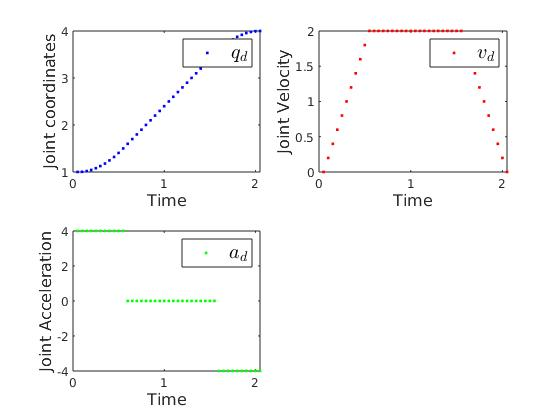
\includegraphics[width=0.8\textwidth]{12} % File
	\caption{The joint trajectory from $q(0) = 1$ to $q(2) = 4$ (trapezoidal)} % Name
	\label{fig:mesh3}
\end{figure}

{\centering
\subsection*{Velocity profile of the type $\dot{q}(t) = a(b + sin(ct))$}
}
\addcontentsline{toc}{subsection}{\protect\numberline{}Velocity profile of the type $\dot{q}(t) = a(b + sin(ct))$}%

To solve this task I needed to calculate differential and integral of $\dot{q}(t)$ to obtain $\ddot{q}(t)$ and $q(t)$.
\begin{itemize}
	\item $\dot{q}(t) = a(b + sin(ct))$
	\item $\ddot{q}(t) = ca\cos(ct))$
	\item $q(t) = a(bt - \frac{cos(ct)}{c})+C_0$
	
\end{itemize}

I used function \textbf{solve()} in MATLAB to solve the system of equations including all the constraints.

The result you can see in the figure \ref{fig:mesh4}.

\begin{figure}[H]
	\centering
		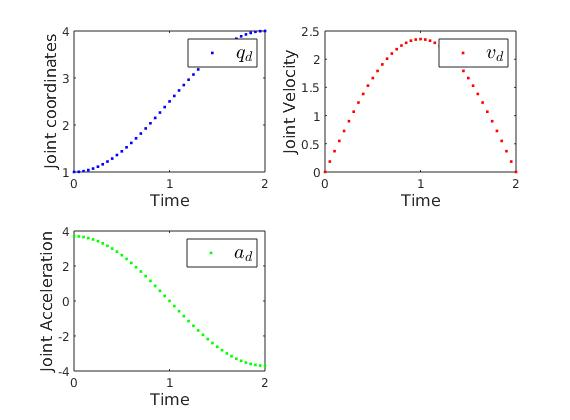
\includegraphics[width=0.8\textwidth]{13} % File
	\caption{The joint trajectory from $q(0) = 1$ to $q(2) = 4$ ($\dot{q(t)} = a(b + sin(ct))$)} % Name
	\label{fig:mesh4}
\end{figure}

\section*{Task 2} \label{sec:Task 2}
\addcontentsline{toc}{section}{\protect\numberline{}Task2}%

Compute the joint trajectory through points $q(0) = 1$, $q(2) = 2$, $q(4) = 0$
with null initial and final velocities and accelerations.
\begin{enumerate}
	\item  Use polynomial position profile
	\item  Use trapezoidal velocity profile.
	\item  Use splines
\end{enumerate}

{\centering
\subsection*{Polynomial Position Profile}
}
\addcontentsline{toc}{subsection}{\protect\numberline{}Polynomial position profile}%

I have here 7 constraints, so, I need to use polynomial of power 6. And the idea of calculating the coefficients is the same as in subsection \nameref{sec: 1Poly}{}.

The result you can see in the figure \ref{fig:mesh5}.

\begin{figure}[H]
	\centering
		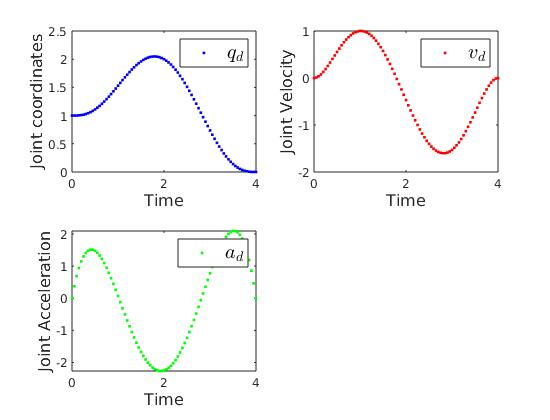
\includegraphics[width=0.8\textwidth]{21} % File
	\caption{joint trajectory through points $q(0) = 1$, $q(2) = 2$, $q(4) = 0$ (polynomial)} % Name
	\label{fig:mesh5}
\end{figure}

{\centering
\subsection*{Trapezoidal Velocity Profile}
}
\addcontentsline{toc}{subsection}{\protect\numberline{}Trapezoidal Velocity Profile}%

Here I had 7 constraints, so I needed to divide the interval into 2 subintervals and make 2 trapezoidal velocity profiles there to satisfy the constraints. The idea is the same as in subsection \nameref{sec: 1Trap}{}
So, equations for my trajectory are:

\begin{equation}
q = \begin{cases} 
      a_{10} + a_{11}t + a_{12}t^2 & t_0 \leq t \leq t_0 + t_b \\
      V_1t + C_1 & t_0 + t_b < t \leq t_1 - t_b \\
      a_{20} + a_{21}t + a_{22}t^2 & t_1 - t_b \leq t \leq t_1 \\
      a_{30} + a_{31}t + a_{32}t^2 & t_1 \leq t \leq t_1 + t_b \\
      V_2t + C_2 & t_1 + t_b < t \leq t_f - t_b \\
      a_{40} + a_{41}t + a_{42}t^2 & t_f - t_b \leq t \leq t_f 

\end{cases}
\end{equation}

The results you can see in the figure \ref{fig:mesh6}.

\begin{figure}[H]
	\centering
		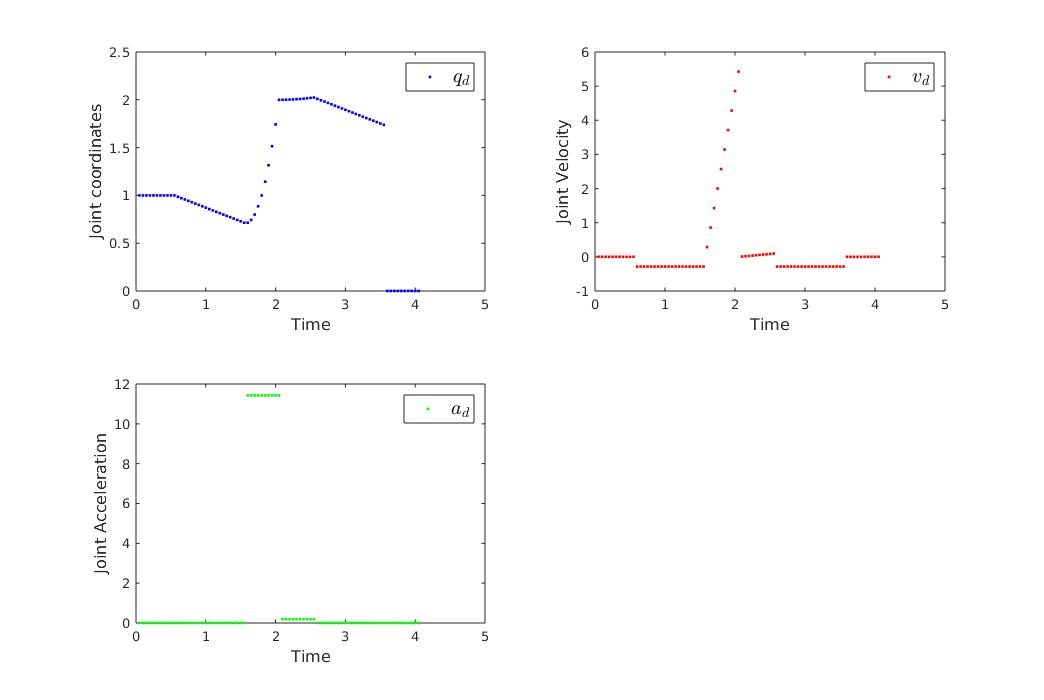
\includegraphics[width=0.8\textwidth]{22} % File
	\caption{joint trajectory through points $q(0) = 1$, $q(2) = 2$, $q(4) = 0$ (trapezoidal)} % Name
	\label{fig:mesh6}
\end{figure}


{\centering
\subsection*{Splines}
}
\addcontentsline{toc}{subsection}{\protect\numberline{}Splines}%

An alternative to using a single high order polynomial for the entire trajec-
tory is to use low order polynomials for trajectory segments between adjacent
via points. These polynomials sometimes refered to as interpolating polyno-
mials or blending polynomials. With this approach, we must take care that
continuity constraints (e.g., in velocity and acceleration) are satisfied at the via
points, where we switch from one polynomial to another.

For example, given initial and final times, $t_0$ and $t_f$, respectively, with 

\begin{equation}
	q^d(t_0) = q_0	;	q^d(t_f) = q_1
	\dot{q}^d(t_0) = q'_0	;	\dot{q}^d(t_f) = q'_1
\end{equation}

the required cubic polynomial q d (t) can be computed from

\begin{equation}
	q^d(t_0) = a_0 + a_1(t-t_0) + a_2(t-t_0)^2 +a_3(t-t_0)^3
\end{equation}

where 

\begin{equation}
	a_2 = \frac{3(q_1-q_0)-(2q'_0+q'1)(t_f-t_0)}{(t_f-t_0)^2}
\end{equation}


\begin{equation}
	a_3 = \frac{2(q_0-q_1)+(q'_0+q'1)(t_f-t_0)}{(t_f-t_0)^3}
\end{equation}

I had also constraints about acceleration, so I needed to use polynomials of power equal to three and five.

\begin{equation}
	q = \begin{cases}
	a_{00} + a_{01}(t) + a_{02}(t)^2 +a_{03}(t)^3 & t_0 \leq t \leq t_1 \\
	a_{10} + a_{11}(t) + a_{12}(t)^2 +a_{13}(t)^3+a_{14}(t)^4++a_{15}(t)^5  & t_1 \leqslant t \leq t_f
	\end{cases}
\end{equation}

The results you can see in the figure \ref{fig:mesh7}.

\begin{figure}[H]
	\centering
		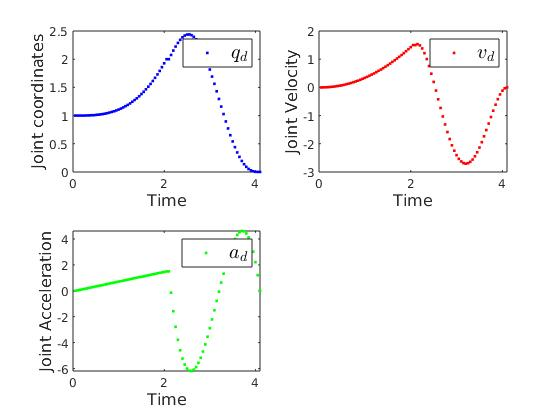
\includegraphics[width=0.8\textwidth]{23} % File
	\caption{joint trajectory through points $q(0) = 1$, $q(2) = 2$, $q(4) = 0$ (Splines)} % Name
	\label{fig:mesh7}
\end{figure}

\section*{Results} \label{sec:Results}
\addcontentsline{toc}{section}{\protect\numberline{}Results}%

Let me compare different approaches that I used in both tasks.

\begin{table}[H]
\centering
\begin{tabular}{ |c||c||c||c||c| }
 \hline
 \multicolumn{5}{|c|}{Table of Max, Min $\dot{q}(t)$, $\ddot{q}(t)$} \\
 \hline
 Method & $\dot{q}_min(t)$ & $\dot{q}_max(t)$ & $\ddot{q}_min(t)$ & $\ddot{q}_max(t)$\\
 \hline
 $POLYNOMIAL_1$ & 0 & 2.2 & -4.5 & 4.5\\
 $TRAPEZOIDAL_1$ & 0 & 2 & -4 & 4\\
 $\dot{q}(t) = a(b + sin(ct))$ & 0 & 2.3 & -3.7 & 3.7\\
 $POLYNOMIAL_2$ & -1.6 & 1 & -2.3 & 2.1\\
 $TRAPEZOIDAL_2$ & -1.3 & 0.6 & -2.6 & 2.6\\
 $SPLINE$ & -2.7 & 1.5 & -6.2 & 4.6\\
 \hline
\end{tabular}
\caption{Methods Comparison}
\label{table:1}
\end{table}
 
 As I concluded, with bigger amount of constraints spline is more unsufficient and enegry expensive than other methods (see \ref{table:1}). Sine law also makes robot move too fast what can affect on energy efficiency. Polynomial ones give smooth enough result and low energy consumption. Also, spline has fast changing for jerk, that can damage the construction.
 

\end{document}